\documentclass[12pt,a4paper]{article}
\usepackage{amsmath,amssymb}
\usepackage{graphicx}
\usepackage{geometry}
\usepackage{float}
\usepackage{booktabs}
\usepackage{xcolor}
\usepackage{hyperref}

\usepackage{xepersian}

\settextfont{B-NAZANIN.TTF} 
\setlatintextfont[Scale=0.85]{Times New Roman}

\renewcommand{\labelitemi}{$\bullet$}
\renewcommand{\labelitemii}{$\circ$}

\title{گزارش پروژه چهارم بینایی \lr{GPS, IMU, EKF}}
\author{استاد درس:‌ دکتر جوانمردی، دکتر خادمیان \\ امیررضا کاظم لو \\ \small درس ربات‌های متحرک خودگردان \\}
\date{\today}

\begin{document}
	\maketitle
	


\section*{دسترسی به کدها و داده‌های پروژه}

\begin{itemize}
	\item \textbf{ گیت‌هاب (کدهای منبع):} \\
	\lr{\href{https://github.com/amirreza1998/-Autonomous-Mobile-Robot/robot-forth-assignment}{https://github.com/amirreza1998/-Autonomous-Mobile-Robot/robot-forth-assignment}}
\end{itemize}
\vspace{0.5cm}

	
\section{تبدیل مختصات جغرافیایی به دکارتی (\lr{ENU})}

برای حل قسمت اول تمرین، ابتدا باید موقعیت‌های \lr{GPS} را از قالب مختصات جغرافیایی (طول و عرض جغرافیایی) به دستگاه مختصات دکارتی \lr{ENU} با تقریب یک صفحه محلی تبدیل می‌کردم. 

طبق فرض مسئله، زمین را به عنوان یک کره با شعاع ثابت در نظر گرفتم. شعاع کره زمین در صورت سوال ۶۴۰۰ کیلومتر داده شده است، اما از آنجایی که در مراحل بعدی برای پیاده‌سازی فیلتر کالمن توسعه‌یافته، داده‌های شتاب‌سنج در فایل \lr{imu.txt} بر حسب واحد $m/s^2$ هستند، تصمیم گرفتم از همین ابتدا برای یکپارچگی واحدها، شعاع کره زمین را به متر ($R=6400000\text{\lr{m}}$) تبدیل کنم. 

با توجه به ساختار فایل \lr{gps.txt} که شامل زمان، عرض و طول جغرافیایی است، داده‌ها را خوانده و ابتدا تمامی مقادیر طول و عرض جغرافیایی را از درجه به رادیان تبدیل کردم. سپس نقطه اول مجموعه داده را به عنوان مبدا مختصات صفحه محلی یعنی $(lat_0, lon_0)$ حول اولین نقطه در نظر گرفتم. در نهایت، با استفاده از روابط داده شده، مختصات دکارتی را محاسبه کردم:

$$x_t=R(lon_t-lon_0)\cos(lat_0)$$
$$y_t=R(lat_t-lat_0)$$

در این روابط، $x_t$ نشان‌دهنده موقعیت در راستای شرق و $y_t$ نشان‌دهنده موقعیت در راستای شمال در صفحه تقریب زده شده است. برای پیاده‌سازی این بخش از کتابخانه \lr{pandas} برای بارگذاری داده‌ها و از \lr{numpy} برای محاسبات سریع و برداری روی کل داده‌ها استفاده کردم. 

جهت صحت‌سنجی درستی محاسبات و کدهای نوشته شده، مسیر حرکت ربات را روی صفحه دو بعدی رسم کردم. همان‌طور که در شکل \ref{fig:trajectory} مشخص است، مسیر تبدیل‌شده به درستی یک حرکت دایره‌ای را نشان می‌دهد که از نقطه مبدا یعنی مختصات $(0,0)$ آغاز شده است.

\begin{figure}[h]
	\centering
	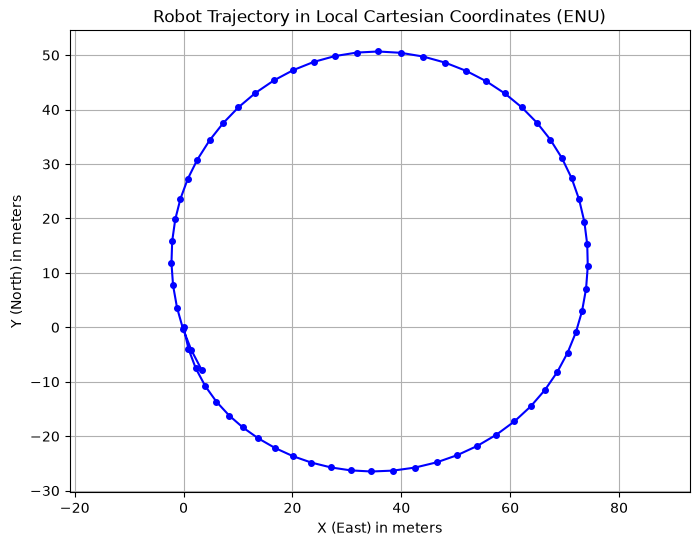
\includegraphics[width=0.7\textwidth]{images/Robot-Trajectory-in-ENU.png}
	\caption{مسیر حرکت ربات در دستگاه مختصات محلی دکارتی (\lr{ENU})}
	\label{fig:trajectory}
\end{figure}


\section{مدل تغییر حالت و مشاهدات}

برای استخراج مدل سینماتیک ربات، باید معادلات حرکت را بر اساس متغیرهای حالت، داده‌های سنسور \lr{IMU} و مشاهدات \lr{GPS} فرمول‌بندی می‌کردم. طبق صحبت های دکتر خادمیان به این مدل کردن میگن \lr{loosly coupled} یعنی ما دیتای خام از سنسور ها دریافت نمی کنیم و به فیلتر مون بدیم بلکه مختصات دقیق را در سنسور ها( این که کجا هستیم) می گیریم.

طبق راهنمایی اول تمرین، بردار حالت سیستم را ۵ بعدی در نظر گرفتم. این بردار شامل موقعیت، سرعت خطی در دستگاه جهانی و زاویه سمت (\lr{Heading}) ربات است:
$$X_t=\begin{bmatrix}x_t\\y_t\\\dot{x}_t\\\dot{y}_t\\\psi_t\end{bmatrix}$$

ورودی‌های سیستم نیز از فایل \lr{IMU} استخراج می‌شوند که شامل شتاب‌های خطی در راستای محورهای بدنه ($\ddot{x}_B,\ddot{y}_B$) و سرعت زاویه‌ای حول محور قائم بدنه ($\dot{\psi}$) هستند:
$$U_t=\begin{bmatrix}\ddot{x}_B\\\ddot{y}_B\\\dot{\psi}\end{bmatrix}$$

\subsection{مدل \lr{System Equation}}
نکته مهم در تشکیل مدل تغییر حالت به فرم $X_t=g(X_{t-1},U_t,\Delta t)+\epsilon$ این است که شتاب‌سنج، مقادیر را در دستگاه مختصات بدنه (\lr{Body Frame}) اندازه‌گیری می‌کند، در حالی که متغیرهای موقعیت و سرعت در بردار حالت در دستگاه مختصات جهانی (\lr{Global Frame}) قرار دارند. بنابراین، ابتدا شتاب‌های بدنه را با استفاده از زاویه $\psi_{t-1}$ به شتاب‌های جهانی ($\ddot{x}_G,\ddot{y}_G$) تصویر کردم:
$$\ddot{x}_G=\ddot{x}_B\cos(\psi_{t-1})-\ddot{y}_B\sin(\psi_{t-1})$$
$$\ddot{y}_G=\ddot{x}_B\sin(\psi_{t-1})+\ddot{y}_B\cos(\psi_{t-1})$$

سپس با استفاده از معادلات پایه سینماتیک، مدل نهایی تغییر حالت را به صورت زیر به دست آوردم:
$$X_t=\begin{bmatrix}x_{t-1}+\dot{x}_{t-1}\Delta t+\frac{1}{2}(\ddot{x}_B\cos\psi_{t-1}-\ddot{y}_B\sin\psi_{t-1})\Delta t^2\\y_{t-1}+\dot{y}_{t-1}\Delta t+\frac{1}{2}(\ddot{x}_B\sin\psi_{t-1}+\ddot{y}_B\cos\psi_{t-1})\Delta t^2\\\dot{x}_{t-1}+(\ddot{x}_B\cos\psi_{t-1}-\ddot{y}_B\sin\psi_{t-1})\Delta t\\\dot{y}_{t-1}+(\ddot{x}_B\sin\psi_{t-1}+\ddot{y}_B\cos\psi_{t-1})\Delta t\\\psi_{t-1}+\dot{\psi}\Delta t\end{bmatrix}+\epsilon$$

\subsection{مدل \lr{Observation Model}}
بر اساس راهنمایی دوم تمرین، موقعیت تبدیل‌شده \lr{GPS} (مؤلفه‌های $x$ و $y$) را مستقیماً به عنوان مشاهده در نظر گرفتم. از آنجا که مشاهدات صرفاً استخراج مستقیم دو متغیر اول از بردار حالت هستند، مدل کاملاً خطی خواهد بود. 

بردار مشاهدات ۲ بعدی به فرم زیر است:
$$Y_t=\begin{bmatrix}x_{gps}\\y_{gps}\end{bmatrix}$$

مدل مشاهدات را به صورت $Y_t=HX_t+\delta$ تعریف کردم که در آن $H$ ماتریس مشاهدات با ابعاد ۲ در ۵ است. این ماتریس فقط $x_t$ و $y_t$ را استخراج می‌کند:
$$Y_t=\begin{bmatrix}1&0&0&0&0\\0&1&0&0&0\end{bmatrix}\begin{bmatrix}x_t\\y_t\\\dot{x}_t\\\dot{y}_t\\\psi_t\end{bmatrix}+\delta$$



البته بد نیست اینجا به یک نکته هم اشاره کنم؛ همان‌طور که سر کلاس دکتر خادمیان مطرح کردند، ایده جالب‌تری هم برای مدل مشاهدات وجود داشت. می‌توانستم شتاب و سرعت زاویه‌ای رو با استفاده از تفاضل‌گیری مقادیر حالت در دو یا سه گام زمانی قبل (\lr{Time Steps}) تخمین بزنم و آن‌ها رو به عنوان متغیرهای تاخیردار توی مشاهدات قرار بدم. این کار قاعدتاً به فیلتر کمک می‌کرد تا تاریخچه حرکت ربات رو بهتر درک کنه و کمی از اثر نویزهای لحظه‌ای کم بشه.

اما خب، از آنجایی که توی راهنمایی دوم صورت سوال پیشنهاد شده بود که فقط موقعیت \lr{GPS} رو مستقیم به عنوان مشاهده در نظر بگیرم تا مدل خطی بمونه، من هم تصمیم گرفتم مسیر منطبق بر خواسته سوال رو انتخاب کنم.

\section{ماتریس ژاکوبین مدل تغییر حالت}

برای قدم بعدی در فیلتر کالمن توسعه‌یافته (\lr{EKF})، باید مدل غیرخطی تغییر حالت رو حول نقطه فعلی (یعنی تخمین قبلی سیستم) خطی‌سازی می‌کردم. این کار با محاسبه ماتریس ژاکوبین نسبت به بردار حالت $X_{t-1}$ انجام می‌شود. محاسبه این ماتریس برای آپدیت کردن ماتریس کواریانس خطا در مرحله \lr{Prediction} مهم است، چون میزان عدم قطعیت مدل ما رو تو هر گام زمانی مشخص می‌کنه.

با توجه به تابع $g(X_{t-1}, U_t, \Delta t)$ که در بخش قبل به دست آوردم، ماتریس ژاکوبین ۵ در ۵ به صورت زیر تعریف می‌شود:

$$F_t = \frac{\partial g}{\partial X_{t-1}} = \begin{bmatrix}
	\frac{\partial x_t}{\partial x_{t-1}} & \frac{\partial x_t}{\partial y_{t-1}} & \frac{\partial x_t}{\partial \dot{x}_{t-1}} & \frac{\partial x_t}{\partial \dot{y}_{t-1}} & \frac{\partial x_t}{\partial \psi_{t-1}} \\
	\frac{\partial y_t}{\partial x_{t-1}} & \frac{\partial y_t}{\partial y_{t-1}} & \frac{\partial y_t}{\partial \dot{x}_{t-1}} & \frac{\partial y_t}{\partial \dot{y}_{t-1}} & \frac{\partial y_t}{\partial \psi_{t-1}} \\
	\frac{\partial \dot{x}_t}{\partial x_{t-1}} & \frac{\partial \dot{x}_t}{\partial y_{t-1}} & \frac{\partial \dot{x}_t}{\partial \dot{x}_{t-1}} & \frac{\partial \dot{x}_t}{\partial \dot{y}_{t-1}} & \frac{\partial \dot{x}_t}{\partial \psi_{t-1}} \\
	\frac{\partial \dot{y}_t}{\partial x_{t-1}} & \frac{\partial \dot{y}_t}{\partial y_{t-1}} & \frac{\partial \dot{y}_t}{\partial \dot{x}_{t-1}} & \frac{\partial \dot{y}_t}{\partial \dot{y}_{t-1}} & \frac{\partial \dot{y}_t}{\partial \psi_{t-1}} \\
	\frac{\partial \psi_t}{\partial x_{t-1}} & \frac{\partial \psi_t}{\partial y_{t-1}} & \frac{\partial \psi_t}{\partial \dot{x}_{t-1}} & \frac{\partial \psi_t}{\partial \dot{y}_{t-1}} & \frac{\partial \psi_t}{\partial \psi_{t-1}}
\end{bmatrix}$$

با مشتق‌گیری جزئی از تک‌تک معادلات تغییر حالت نسبت به متغیرهای $\left[x, y, \dot{x}, \dot{y}, \psi\right]$، ماتریس نهایی رو به این شکل محاسبه کردم:

$$F_t = \begin{bmatrix}
	1 & 0 & \Delta t & 0 & \frac{1}{2}(-\ddot{x}_B\sin\psi_{t-1} - \ddot{y}_B\cos\psi_{t-1})\Delta t^2 \\
	0 & 1 & 0 & \Delta t & \frac{1}{2}(\ddot{x}_B\cos\psi_{t-1} - \ddot{y}_B\sin\psi_{t-1})\Delta t^2 \\
	0 & 0 & 1 & 0 & (-\ddot{x}_B\sin\psi_{t-1} - \ddot{y}_B\cos\psi_{t-1})\Delta t \\
	0 & 0 & 0 & 1 & (\ddot{x}_B\cos\psi_{t-1} - \ddot{y}_B\sin\psi_{t-1})\Delta t \\
	0 & 0 & 0 & 0 & 1
\end{bmatrix}$$

همان‌طور که در صورت تمرین هم به درستی پیشنهاد شده بود، برای پیاده‌سازی راحت‌تر و اصولی‌تر این بخش توی کدم، یک تابع پایتون مجزا تعریف کردم. کار این تابع اینه که هر بار مقادیر نقطه مشتق‌گیری (یعنی تخمین فعلی حالت و شتاب‌های خوانده‌شده از \lr{IMU}) رو به همراه اختلاف زمان $\Delta t$ بگیره و این ماتریس ۵ در ۵ رو خروجی بده. اینطوری هر بار که فیلتر کالمن در مرحله \lr{Prediction} فراخوانی میشه، ماتریس ژاکوبین به‌صورت کاملاً دینامیک و بر اساس جدیدترین وضعیت ربات محاسبه و جایگذاری میشه.
این ماتریس را در تابع \lr{calculate\_jacobian\_F} پیاده سازی کردم.ورودی های تابع مقادیر زیر هستند:
\begin{itemize}
	\item \lr{X\_prev} (\lr{numpy.ndarray}): بردار حالت قبلی $[x, y, v_x, v_y, \psi]$
	\item \lr{U\_t} (\lr{numpy.ndarray}): بردار ورودی فعلی $[ax_B, ay_B, \omega]$
	\item \lr{dt} (\lr{float}): گام زمانی ($\Delta t$)
\end{itemize}

\section{پیاده‌سازی مرحله ‌ \lr{Update}}

همان‌طور که در صورت تمرین اشاره شده بود، از آنجا که موقعیت گرفته‌شده از \lr{GPS} را مستقیماً به عنوان مشاهده در نظر گرفتم، مدل مشاهدات من کاملاً خطی است. این خطی بودن کار را بسیار ساده می‌کند، زیرا ماتریس مشاهدات ($H$) یک ماتریس ثابت است و در مرحله به‌روزرسانی نیازی به خطی‌سازی مجدد و محاسبه ژاکوبین برای بخش مشاهدات ندارم. و معادلات آن خطی کالمن استاندارد می شود.



ابتدا \lr{Innovation} را که تفاضل بین مقدار اندازه‌گیری‌شده توسط سنسور و مقدار پیش‌بینی‌شده توسط مدل است، محاسبه کردم:
$$y_t = Z_t - H X_{pred}$$

سپس ماتریس کواریانس باقیمانده ($S_t$) را به دست آوردم. در فرمول زیر $Q$ نویز مشاهده است:
$$S_t = H P_{pred} H^T + Q_{obs}$$

در قدم بعدی، \lr{Kalman Gain} را محاسبه کردم تا مشخص شود چقدر باید به مشاهدات جدید در مقابل پیش‌بینیِ مدل اعتماد کنم:
$$K_t = P_{pred} H^T S_t^{-1}$$

در نهایت، با استفاده از بهره‌ی کالمن، بردار حالت و ماتریس کواریانسِ \lr{belief} سیستم را به‌روزرسانی کردم:
$$X_{upd} = X_{pred} + K_t y_t$$
$$P_{upd} = (I - K_t H) P_{pred}$$
در کد این بخش ها در تابع \lr{update(X\_pred, P\_pred, Z\_meas, H, Q\_obs)} پیاده سازی شده است که $$P_{upd} , X_{upd}$$ را در خروجی دارد.

\section{تعیین ماتریس‌های نویز و تخمین حالت اولیه}

\subsection{ماتریس‌های کواریانس نویز}
برای مدل‌سازی عدم قطعیت در سیستم، ماتریس‌های کواریانس نویز مدل ($R$) و مشاهدات ($Q$) به صورت زیر می‌باشد:

$$R = \begin{bmatrix}
	100 & 0 & 0 & 0 & 0 \\
	0 & 100 & 0 & 0 & 0 \\
	0 & 0 & 16 & 0 & 0 \\
	0 & 0 & 0 & 16 & 0 \\
	0 & 0 & 0 & 0 & 0.25
\end{bmatrix}, \quad
Q = \begin{bmatrix}
	100 & 0 \\
	0 & 100
\end{bmatrix}$$

\subsection{تخمین تحلیلی حالت اولیه ($X_0$)}
برای راه‌اندازی فیلتر کالمن (\lr{Initialization})، نیاز به یک تخمین اولیه از بردار حالت داشتم. از آنجایی که در لحظه شروع هیچ تخمین قبلی وجود نداشت، از دو نقطه متوالی داده‌های \lr{GPS} (سطر اول و دوم مجموعه داده) استفاده کردم تا این مقادیر را به‌صورت دستی و تحلیلی محاسبه کنم. 

داده‌های خام دو نقطه اول \lr{GPS} به این شرح است:
\begin{itemize}
	\item \textbf{نقطه صفر ($t_0$):} زمان = $1703098100.378$ ثانیه، عرض = $47.639488^\circ$، طول = $-122.150120^\circ$
	\item \textbf{نقطه یک ($t_1$):} زمان = $1703098100.587$ ثانیه، عرض = $47.639453^\circ$، طول = $-122.150108^\circ$
\end{itemize}

اختلاف زمانی بین این دو خوانش $\Delta t = 0.2084$ ثانیه بود. با قرار دادن نقطه صفر به عنوان مبدا مختصات صفحه محلی (\lr{ENU})، مقادیر اولیه $x_0 = 0$ و $y_0 = 0$ در نظر گرفته شدند.

سپس نقطه دوم را با استفاده از روابط قبلی به دستگاه \lr{ENU} تبدیل کردم:
$$x_1 = 6400000 \times (-122.150108 - (-122.150120)) \times \frac{\pi}{180} \times \cos(47.639488^\circ) \approx 0.8941 \text{ \lr{m}}$$
$$y_1 = 6400000 \times (47.639453 - 47.639488) \times \frac{\pi}{180} \approx -3.9263 \text{ \lr{m}}$$

با فرض حرکت بدون شتاب (تقریبا درسته چون بازه زمانی خیلی کوچیک هست قابل اغماض هست)، سرعت‌های اولیه در راستای $x$ و $y$ به صورت زیر می شود:
$$\dot{x}_0 = \frac{x_1 - x_0}{\Delta t} = \frac{0.8941}{0.2084} \approx 4.2908 \text{ \lr{m/s}}$$
$$\dot{y}_0 = \frac{y_1 - y_0}{\Delta t} = \frac{-3.9263}{0.2084} \approx -18.8423 \text{ \lr{m/s}}$$

در نهایت، زاویه \lr{Heading} اولیه با استفاده از تانژانت برعکس سرعت ها در این دو جهت به‌دست میاد:
$$\psi_0 = \operatorname{atan2}(\dot{y}_0, \dot{x}_0) = \operatorname{atan2}(-18.8423, 4.2908) \approx -1.3467 \text{ \lr{rad}}$$

بنابراین، بردار حالت اولیه ($X_0$) برای شروع فیلتر کالمن به صورت می شود:
$$X_0 = \begin{bmatrix} 0 \\ 0 \\ 4.2908 \\ -18.8423 \\ -1.3467 \end{bmatrix}$$


در کد، تابعی به نام \lr{\texttt{initialize\_state}} تعریف کردم. ورودی‌های این تابع شامل دو سطر اول از داده‌های \lr{GPS} (که حاوی زمان، عرض و طول جغرافیایی هستند) و همچنین مقدار ثابت شعاع زمین ($R$) است. در داخل این تابع، ابتدا زمان‌ها که بر حسب نانوثانیه ثبت شده‌اند به ثانیه تبدیل می‌شوند تا با واحد متر بر ثانیه در سرعت‌ها هم‌خوانی داشته باشند. سپس دقیقا همین روابط که به صورت دستی حساب کردم رو اونجا به صورت کد پیاده کردم. که خروجی بردار حالت $X_0$ را برای شروع حلقه اصلی فیلتر کالمن برمی‌گرداند.
خروجی آن به صورت زیر شده است که مطابق محاسبات دستی من هست:
\begin{figure}[H]
	\centering
	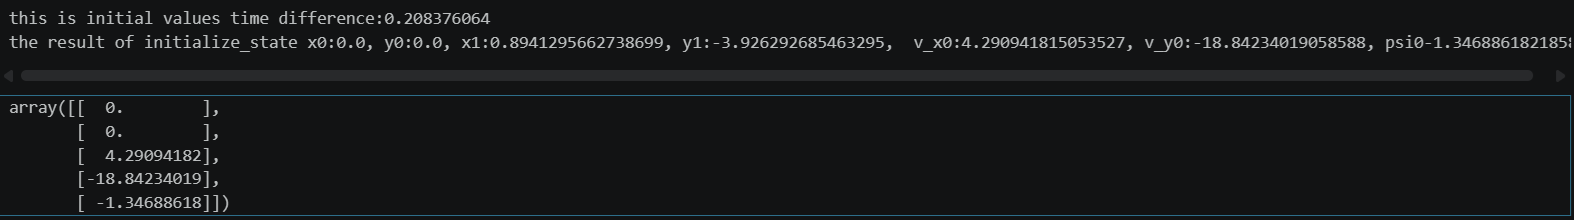
\includegraphics[width=1.2\textwidth]{images/code-result-initialization.png}
\end{figure}


\section{اجرای حلقه اصلی فیلتر بیز (\lr{Prediction \& Update})}

برای اجرای حلقه اصلی فیلتر کالمن توسعه‌یافته، باید داده‌های سنسورها را به‌صورت متوالی و بر اساس زمان وقوع آن‌ها پردازش می‌کردم. از آنجا که نرخ تولید داده در سنسور \lr{IMU} به‌مراتب بیشتر از سنسور \lr{GPS} است و برچسب‌های زمانی (\lr{Timestamps}) این دو سنسور دقیقاً بر هم منطبق نیستند، پس داده‌های هر دو سنسور را ادغام کردم و بر اساس زمان مرتب کنم. 

مراحل پیاده‌سازی:

\begin{enumerate}
	\item ابتدا داده‌های \lr{IMU} و \lr{GPS} که قبل از زمان $t_1$ (زمان دومین داده‌ی \lr{GPS} که برای تخمین حالت اولیه $X_0$ استفاده شد) بودند را از مجموعه داده‌ها حذف کردم. سپس هر دو مجموعه داده را در یک ساختار واحد ترکیب کرده و بر اساس ستون \lr{Timestamp} به صورت صعودی مرتب کردم. یه ستون هم در \lr{pandas} ایجاد کردم که مشخص می کرد نوع دیتا از نوع \lr{IMU}هست و یا \lr{GPS}.
	
	\item بردار حالت ($X_0$) را برابر با خروجی مرحله‌ی قبل قرار دادم. همچنین ماتریس کواریانس اولیه ($P_0$) را با مقادیر نسبتاً کوچکی در قطر اصلی (مثلاً ماتریس همانی) مقداردهی کردم، زیرا به تخمین تحلیلی اولیه اطمینان داریم چون حساب کردیم خودمون.
	
	\item روی لیست داده‌های مرتب‌شده یک \lr{loop} ایجاد کردم. در هر تکرار، ابتدا اختلاف زمان ($\Delta t$) نسبت به داده‌ی قبلی را بر حسب ثانیه محاسبه کردم. سپس بر اساس نوع داده، یکی از دو گام زیر را اجرا کردم:
	\begin{itemize}
		\item \textbf{نوع داده \lr{IMU}:} گام پیش‌ \lr{Prediction} را میریم. در این گام، ماتریس ژاکوبین ($F_t$) حول نقطه فعلی محاسبه می کنم، بردار حالت با استفاده از معادلات  غیرخطی ($g$) رو به جلو هدایت شد و در نهایت ماتریس کواریانس باور ($P$) با اضافه کردن نویز مدل ($R$) بدست میاد.
		\item \textbf{نوع داده \lr{GPS}:} گام  \lr{Update} را میریم. در این گام، موقعیت‌های $x$ و $y$ اندازه‌گیری شده در دستگاه \lr{ENU} و با استفاده از معادلات خطی فیلتر کالمن، بهره‌ی کالمن ($K$) حسابمی کنم. بعد بردار حالت و ماتریس کواریانس با در نظر گرفتن ماتریس نویز مشاهدات ($Q$) تصحیح می شن.
	\end{itemize}
\end{enumerate}

همان‌طور که انتظار می‌رفت، به دلیل فرکانس بالاتر سنسور \lr{IMU}، در بیشتر تکرارهای تنها فاز پیش‌بینی اجرا می‌شد و ماتریس عدم قطعیت سیستم بزرگتر میشه، و هر زمان که داده‌ی \lr{GPS} در دسترس قرار می‌گرفت، فاز به‌روزرسانی اجرا شده و عدم قطعیت تصحیح و کاهش می‌یافت. در نهایت تمامی بردارهای حالت و ماتریس‌های کواریانس در طول زمان در \lr{history} ذخیره می کنم.

\section{ترسیم خروجی‌های فیلتر}

پس از پیاده‌سازی و اجرای تابع \lr{\texttt{run\_ekf}} بر روی داده‌ها \lr{history} حاصل از \lr{EKF} را رسم می کنم که در تابع \lr{plot\_covariance\_ellipse} پیاده شده.

در شکل \ref{fig:ekf_result} سه مؤلفه اصلی را در یک صفحه مختصات دو بعدی نمایش داده‌ام:
\begin{itemize}
	\item \textbf{نقاط قرمز رنگ (\lr{GPS Observations}):} این نقاط نمایانگر مشاهدات خام سنسور \lr{GPS} پس از انتقال به دستگاه مختصات محلی \lr{ENU} هست.
	\item \textbf{خط آبی رنگ (\lr{EKF Belief Mean}):} این خطِ پیوسته، میانگین توزیع باور یا همان مسیر تخمینی نهایی ربات است که توسط فیلتر کالمن محاسبه شده است. فیلتر تونسته یک مسیر دایره‌ای و بسیار هموار را از بین داده‌های نویزی استخراج کند.
	\item \textbf{بیضی‌های سبز رنگ (\lr{Belief Covariance Contour}):} این کانتورها نشان‌دهنده حاشیه عدم قطعیت فیلتر (با تقریب یک انحراف معیار یا $1\sigma$) در هر لحظه هستند. 
\end{itemize}


شعاعِ بزرگ بیضی‌های عدم قطعیت (کانتورهای سبز) نسبت به خود مسیر حرکت است. دلیل این پدیده، مقادیری است که در متن تمرین برای ماتریس‌های نویز تعریف شده بود. مقادیر واریانسِ موقعیت در ماتریس نویز فرآیند ($R$) و ماتریس نویز مشاهدات ($Q$) هر دو عدد نسبتاً بزرگی ($100 \^2$) فرض شده‌اند، سیستم به طور ذاتی با عدم قطعیت بالایی (انحراف معیار حدود ۱۰ متر در هر محور) مدل شده است. 

در فواصل زمانی بین دریافت دو داده‌ی متوالی \lr{GPS}، فیلتر با استفاده از داده‌های \lr{IMU} در گام \lr{Prediction} مسیر را پیش‌بینی می‌کند که باعث رشد این بیضی‌ها می‌شود. با رسیدن داده‌ی \lr{GPS} جدید (گام \lr{Update})، فیلتر عدم قطعیت را کاهش می‌دهد؛ اما به دلیل بزرگ بودن نویز اندازه‌گیری ($Q$)، این عدم قطعیت هیچ‌گاه از یک حد مشخصی کمتر نمی‌شود و به همین دلیل کانتورها در کل مسیر نسبتاً بزرگ باقی مانده‌اند.

\begin{figure}[htbp]
	\centering
	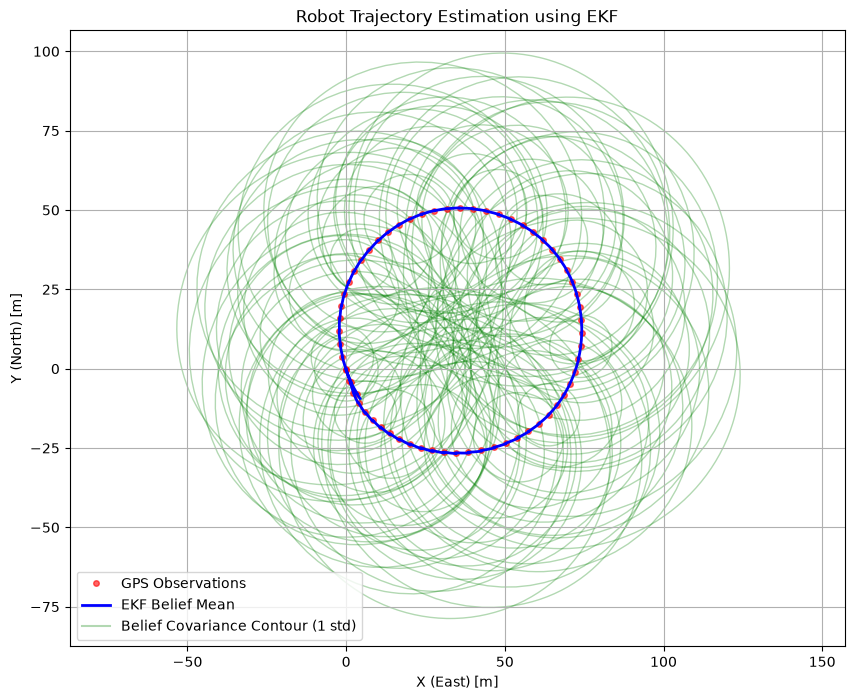
\includegraphics[width=0.9\textwidth]{images/efk-result-plot.png}
	\caption{تخمین مسیر حرکت ربات با استفاده از \lr{EKF}؛ مقایسه مشاهدات \lr{GPS}، مسیر تخمینی و کانتورهای عدم قطعیت}
	\label{fig:ekf_result}
\end{figure}


\section{ افزایش نویز مشاهدات به ۱۰۰ متر}

انحراف معیار نویز مشاهدات را به ۱۰۰ متر در هر بُعد افزایش دادم و فیلتر را مجدداً روی داده‌ها اجرا کردم. 

از آنجا که ماتریس کواریانس مشاهدات ($Q$) بیانگر واریانس است، برای رسیدن به انحراف معیار ۱۰۰ متر، درایه‌های قطر اصلی را در کد برابر با $100^2 = 10000$ تنظیم کردم:
$$Q_{new} = \begin{bmatrix}
	10000 & 0 \\
	0 & 10000
\end{bmatrix}$$

پس از اجرای مجدد الگوریتم با این ماتریسِ تغییریافته، خروجی مطابق با شکل \ref{fig:ekf_q10000} رسیدم.

\begin{itemize}
	\item \textbf{رشد بسیار شدید عدم قطعیت (بزرگ شدن کانتورها):} کانتورهای ماتریس کواریانس به شدت پهناور شده‌اند و شعاع آن‌ها به صورت بصری با مقیاس ۱۰۰ متر تطابق دارد. نشان می‌ده که سیستم به دلیل خطای بالای تعریف‌شده برای سنسور \lr{GPS}، به شدت دچار عدم قطعیت است. در واقع گام به‌روزرسانی قدرت کافی برای خنثی کردن خطای انباشته‌شده در فاز پیش‌بینی را ندارد.
	\item \textbf{افت شدید \lr{Kalman Gain}:} واریانس بسیار بالای مشاهدات باعث می‌شود که مخرج کسر در رابطه محاسبه بهره کالمن به‌شدت بزرگ شود و در نتیجه بهره کالمن کم شود. این یعنی فیلتر برای تصحیح وضعیت خود، وزن بسیار ناچیزی به داده‌های جدید \lr{GPS} می‌دهد.
	\item \textbf{تکیه مطلق بر (\lr{IMU}):} با بی‌اعتماد شدن فیلتر به مشاهدات \lr{GPS}، بار اصلیِ تخمین مسیر بر دوش پیش‌بینی‌های شتابسنج و ژیروسکوپ می‌افتد. به همین دلیل، مسیر تخمینی میانگین باور هموار (\lr{Smooth}) شده است و فیلتر واکنش و تمایلی برای اصلاح مسیر خود با نوسانات ریز و پرش‌های نقطه‌ای \lr{GPS} نشان نمی‌دهد.
\end{itemize}

این نشون دهنده اینه که تنظیم پارامترهای ماتریس نویز می‌توانه در فیلتر کالمن مشخص کنه که به سنسنور یا مدل درونی کدوم یکی رو اهمیت بیشتری بهش بده.

\begin{figure}[htbp]
	\centering
	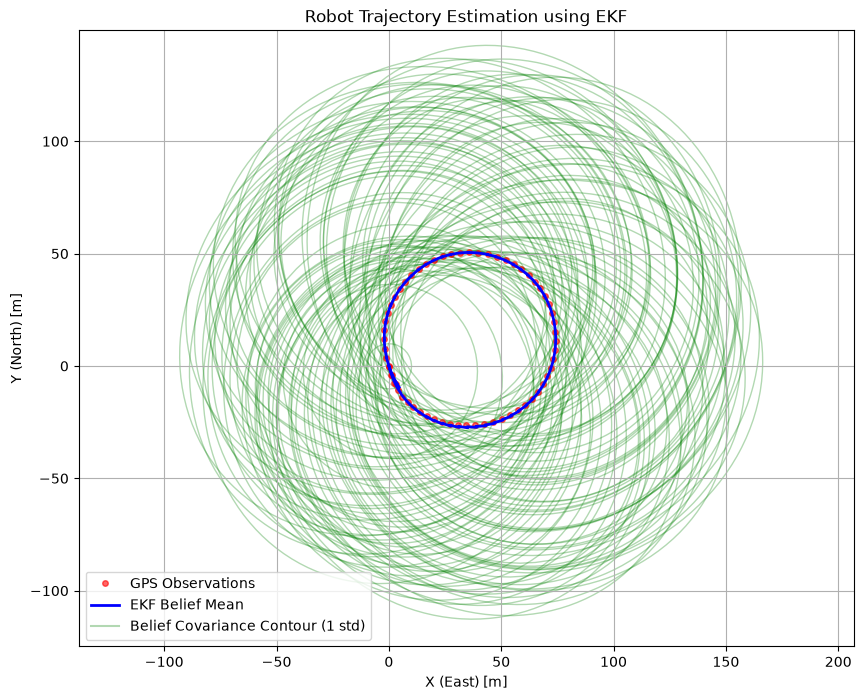
\includegraphics[width=0.9\textwidth]{images/efk-result-plot-Q-increased.png}
	\caption{تخمین مسیر حرکت ربات با افزایش انحراف معیار نویز مشاهدات به ۱۰۰ متر ($Q=10000$)}
	\label{fig:ekf_q10000}
\end{figure}

\end{document}